% !TEX root = ../main.tex

\section{Introduction}
\label{sec:introduction}
In this lab we will find out what striding and warps is all about. We learn how striding is useful in the code execution, why it should be implemented and what the benefits are. The next part of the lab is about warps where we will try to determine the impact of the thread size and limitations of CUDA.

The code repository can be found at: \\
\url{https://github.com/imstevenxyz/geavanceerde-computerarch}

\section{Striding}
\label{sec:striding}

To see the benefits of striding an image is generated using the given formula. This formula is implemented in two kernel functions, one that executes with striding and one without. Both are run with an amount of threads, the total pixels, a quarter of the total pixels and with more than the total pixels.

\begin{figure}[H]
    \centering
    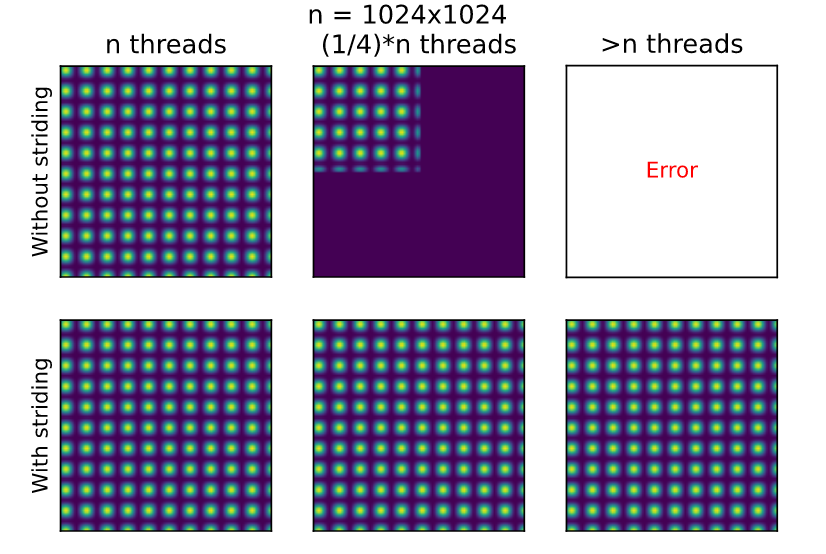
\includegraphics[width=0.5\textwidth]{images/striding.png}
    \caption{Timing performance semi parallel kernel}
    \label{figure:striding}
\end{figure}

It is directly obvious in figure \ref{figure:striding} that without striding we get three different results while with striding we get the wanted result for all variations. The outstanding in the figure is when we use more threads than pixel. In this variation the code will return an error because otherwise memory that does not belong to the image is accessed, this is either impossible or very dangerous (unwanted memory access, data theft, etc). When using a quarter of the pixels, only a quarter of the image is generated because the other pixels will not be calculated since there are not enough threads.

From this we can see that striding actually helps organize the threads in two ways:
\begin{itemize}
    \item Not enough threads? → Run threads sequentially.
    \item More than needed threads? → Do not run the calculations for non-existing memory locations.
\end{itemize}

\section{Warps}
\label{sec:warps}

\section{Conclusion}
\label{sec:conclusion}

